%!TEX program = xelatex
\documentclass[11pt,a4paper]{book}

% Aberstwyth dissertation LaTeX Template
% Authors: Dr. Hannah Dee (hmd1@aber.ac.uk), Neil Taylor (nst@aber.ac.uk)
% This has been adapted from the Leeds Thesis template and the
% Group Project template for Computer Science in Aberystywth University.
%
% All comments and suggestions welcome.
%
% Template designed to be used with pdflatex: it may need alteration to
% run with a different LaTeX engine

% To build document on the unix command line, run four commands:

% pdflatex dissertation
% bibtex dissertation
% pdflatex dissertation
% pdflatex dissertation

% you will end up with dissertation.pdf
\usepackage{mmp}

% the following packages are used for citations - You only need to include one.
%
% Use the cite package if you are using the numeric style (e.g. IEEEannot).
% Use the natbib package if you are using the author-date style (e.g. authordate2annot).
% Only use one of these and comment out the other one.
\usepackage{cite}
%\usepackage{natbib}

% Use the following to selectively exclude chapters
%\includeonly{cover,abstract,acknowledge,declare,chapter1,chapter2}

\newcommand{\todo}[1]{\textcolor{red}{\textbf{\texttt{TODO: #1}}}}
\usepackage{layout}
\begin{document}
% all of the include directives below refer to tex files
% so 
\title{Browser-based Online Multiplayer Roleplaying Game}

% Your name
\author{David Field}

% Your email
\authoremail{dvf9@aber.ac.uk}

\degreeschemecode{G401} %e.g. G400
\degreeschemetitle{Computer Science} % e.g. Computer Science
\degreetype{BSc}

\modulecode{CS39440} % i.e. CS39440, CC39440, CS39620
\moduletitle{Major Project} % i.e. Major Project or Minor Project

\date{\today} % i.e. the date of this version of the report

\status{Draft} % Use draft until you create the release version. Then, change this to Release.
\version{0.1.1}

%The title and name of your supervisor.
\supervisor{Dr. Hannah Dee}

%The email for your supervisor.
\supervisoremail{hmd1@aber.ac.uk}

\maketitle includes cover.tex - to change the content,
% edit the tex file

% \setmainfont[Ligatures=TeX]{Minion Pro}
\pagenumbering{roman}

% \layout
% This is the front page

\title{Browser-based Online Multiplayer Roleplaying Game}

% Your name
\author{David Field}

% Your email
\authoremail{dvf9@aber.ac.uk}

\degreeschemecode{G401} %e.g. G400
\degreeschemetitle{Computer Science} % e.g. Computer Science
\degreetype{BSc}

\modulecode{CS39440} % i.e. CS39440, CC39440, CS39620
\moduletitle{Major Project} % i.e. Major Project or Minor Project

\date{\today} % i.e. the date of this version of the report

\status{Draft} % Use draft until you create the release version. Then, change this to Release.
\version{0.1.1}

%The title and name of your supervisor.
\supervisor{Dr. Hannah Dee}

%The email for your supervisor.
\supervisoremail{hmd1@aber.ac.uk}

\maketitle

% Set up page numbering
\pagestyle{empty}

% declarations of originality
\thispagestyle{empty}

%%%
%%% You must sign the declaration of originality.
%%%
\begin{center}
    {\LARGE\bf Declaration of originality}
\end{center}

In signing below, I confirm that:

\begin{itemize}
\item{This submission is my own work, except where clearly
indicated.  }

\item{I understand that there are severe penalties for plagiarism
and other unfair practice, which can lead to loss of marks
or even the withholding of a degree. }

\item{I have read the sections on unfair practice in the Students'
Examinations Handbook and the relevant sections of the
current Student Handbook of the Department of Computer
Science.}

\item{I understand and agree to abide by the University's
regulations governing these issues.}
\end{itemize}

\vspace{3em}
Signature ............................................................  \\

\vspace{1em}
Date ............................................................ \\

%%%
%%% We would like to make a selection of final reports available to students that take
%%% this module in future years. To enable us to do this, we require your consent. You
%%% are not required that you do this, but if you do give your consent, then we will have
%%% the option to select yours as one of a number of reports as examples for other
%%% students. If you would like to give your consent, then please include the following
%%% text and sign below. If you do not wish to give your consent, please remove this
%%% from your report.
%%%
\vspace{5em}
\begin{center}
    {\LARGE\bf Consent to share this work}
\end{center}

In signing below, I hereby agree to this dissertation being made available to other
students and academic staff of the Aberystwyth Computer Science Department.

\vspace{3em}
Signature ............................................................  \\

\vspace{1em}
Date ............................................................ \\



\thispagestyle{empty}

\begin{center}
    {\LARGE\bf Acknowledgements}
\end{center}

I am grateful to...

I'd like to thank...
 % Acknowledgements
\thispagestyle{empty}

\begin{center}
    {\LARGE\bf Abstract}
\end{center}

% Include an abstract for your project. This should be no more than 300 words.

This report discusses the creation of a game engine that implements isometric graphics, click-based pathfinding movement and multiplayer with multiple running games, hosted in a browser and created with \textsc{html5}, JavaScript and Python with some frameworks.

The report discusses implementation and design details for all the above features, including coordinate conversion, depth sorting and drawing to the screen for the isometric graphics, as well as what isometric is in the context of a game; the creation and following of paths for movement and how those paths are handled when received from remote clients; and how the need for multiple games causes problems in a web-based environment. Particular focus on the server is given to how to create, manage and delete the threads required to run the multiple games; how to route messages to and from these threads and how to connect players to the game in real time on a web platform.                 % Abstract

\pagenumbering{roman}
\pagestyle{fancy}
\fancyhead{}
\fancyfoot[C]{\thepage}
\renewcommand{\headrulewidth}{0 pt}
\renewcommand{\chaptermark}[1]{\markboth{#1}{}}

\tableofcontents
\newpage
\listoffigures
\newpage
\listoftables
\newpage

% Set up page numbering
\pagenumbering{arabic}

\setchapterheaderfooter

% include the chapters
\chapter{Background \& Objectives}

\begin{figure}[H]
    \centering
    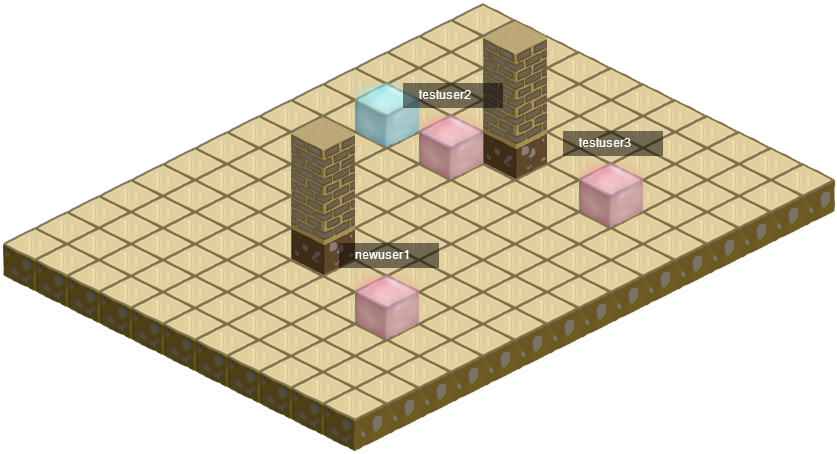
\includegraphics[width=10cm]{Images/the_game.png}
    \caption{The game. Graphics from \cite{GameArt}.}
    \label{fig:the_game}
\end{figure}

Games are interesting projects to take on; they have a history of being difficult to make and pushing technology to its limits. There are a great many systems and features that can be included in them---AI, physics, graphics, audio, UI, multiplayer and more---and a great many ways to implement each, from simple to very complicated depending on the needs of the project.

Games also have a history of aiming for too many of these features in too little time. In most cases, every one of the features thought up would enhance the final product in some way, from a significant improvement that changes the way the game is played to a minor enhancement that makes things just a little more pleasant for the user. Many of these features may be considered mandatory for the game to be worth making at all. For example, a single-player chess game would probably not be very good if there were no AI to play against.

It is clear that, given the sheer enormity of the possible things that can be put into any one game, there is not enough time in this project to implement even half of them without a great deal of previous experience and skill. Every one of the major systems mentioned can be extremely complicated, requiring a lot of research, time and effort to make them work.

This chapter will discuss what the project is; why it was worth taking on; how a minimal system was devised that would satisfy enough of the game design requirements to be playable but also be implementable in the time given; and finally the process used to implement the design requirements.

\section{Background}

\subsection{The Project}
Before discussing the decisions made about what was doable and why it was interesting, it's useful to know what the project actually is.

The name of the project---\textit{Browser-based Online Multiplayer Roleplaying Game}---gives a relatively good hint of the nature of the game. ``Browser-based'' and ``multiplayer'' are fairly self-evident in meaning: multiple people play together in a game hosted in the browser. ``Roleplaying game'' is more ambiguous. In this case, it refers to a game in the style of the classic tabletop roleplaying game \textit{Dungeons \& Dragons.}

In the context of the project that meant the following things: firstly, there needed to be two types of players---regular players and a Game Master. A regular player plays the game as a character inhabiting the world they happen to be in. For example, they may be a dwarf in a fantasy kingdom, or a space marine on a futuristic space station.

The Game Master is a player responsible for building the world, telling the story and controlling characters that aren't controlled by the other players (known as Non-Player Characters or NPCs). Traditionally, the Game Master would also be responsible for enforcing the rules of the world. However, in this project the game was to be responsible for that instead, with the Game Master given the option of overriding or changing the rules if he or she wished to do so.

Combat is the most obvious area where the game enforcing the rules comes into effect. Combat is turn-based, with players put onto a grid and given limits on the distance they can move and number of actions they can perform in each turn. When they attempt to do something---such as attack another character or creature or escape from a trap---they have to roll dice, the result of which decides whether they were successful or not, and how well they succeeded or failed. As an example, a player failing to attack a creature with their sword could simply miss, or they could throw the sword away accidentally, depending on the result of the dice roll.

In the above scenario the dice rolls would be simulated by the game, rather than physical dice being used by the players. The game will also decide whether or not an action was valid in the first place. A player hoping to attack a creature with their sword would be unable to do so if the creature was too far away from them.

The design also called for interactions outside of combat. For instance, a player might be faced with a locked door. To get through a player could attempt to use a key they found or, alternatively, they could attempt to bash the door open with an item, such as an axe, or even their bare hands.

There are a few specific implementation details as well. Apart from the game being played via a browser, there needed to be graphics and those graphics needed to be \textsc{2d} isometric tiles. Further, the server was to be written in Python with the goal of gaining experience in the language.

With this overview of the game it is now important to answer why the project was worth doing.

\subsection{Why Make The Game?}
The first answer to this is that games are interesting in general. Most obviously, the final product of a game is (hopefully) something fun to play with appeal to a wide range of people. More relevant to the context of a project, however, is that games are interesting from a software perspective.

Games are made up of a lot of different parts, each one potentially being difficult to implement by itself. In this game, the most challenging individual parts are graphics and multiplayer. More important than just the individual parts, however, is making sure they integrate properly. In most cases the game needs to share data between these different pieces---game logic needs to know what an object is doing so it can perform game functions on it; the renderer needs to know what the object is doing so that it can be drawn to the screen correctly; the networking part needs to know what the object is doing so that it can forward on any relevant information to the server.

The game also offers a lot of extendibility. Given more time, more features can be added. Each feature, and fitting it together, offers a lot of potential for learning as well. For example, an extra feature could be AI, which is an interesting area in itself that offers a lot of opportunity to learn something new.

\subsection{Reading and Research}
Most of the research in the gaming world is very much a closed source, commercial affair. Being on the cutting edge of games is expensive work, requiring smart people spending a lot of time squeezing everything they can out of technology, plus a whole bunch of people to make content for the technology to show.

Even with the explosion of `indie' games made by one person or a very small team that exist these days, most of them are still closed source and commerical. Even free games are rarely free (and certainly not open source)---existing as a vehicle for microtransactions, asking people to buy consumable cosmetic items or in-game advantages, such as speeding something up, for a small fee.

Of course open source games do exist, though they are relatively rare and not very well known. One of the open source games with most relevance to this project is Mozilla's \textit{BrowserQuest}\cite{citeulike:13139186, citeulike:13139189, citeulike:13139194}, a multiplayer role-playing game created in 2012 to show off the capabilities of modern browsers. It has a few properties that are useful to know for this project, the main one being multiplayer.

However, despite the theoretical usefulness of having access to the source code, it was not as useful in practice as might have been desired or expected. Without documentation that describes the more high level structure of the code it is difficult to read through and understand properly without spending a lot of time on it.

The need to have a higher level overview of structure and concepts leads to books, articles and tutorials.

One of the most popular books available for this is \textit{Game Coding Complete}\cite{citeulike:12394552}. It is a lengthy book but covers a lot of things, both high level and code-specific. Most of the implementation details given are inappropriate for this project because they are for \textsc{3d} graphics, C++ and cover a lot of things like custom memory management that have no equivalent or purpose in a much more simple \textsc{2d}, browser-based game written in JavaScript. However, the high level aspects of game engine design the authors talk about are very useful.

The other major book that was found to be useful in this project is a free book currently available online called \textit{Game Programming Patterns}\cite{citeulike:13049596}. This book describes many common design patterns used in game programming, some being game specific and others being more well known patterns but applied to game programming, such as the classic Factory pattern. Some of the patterns when put together describe a more general structure, in a way similar to \textit{Game Coding Complete.}

The content of these two books informs a great deal of the design that was settled on for this project, with particular emphasis on the central game loop and the event manager. These two fundamental parts of the design act as the glue for the more specific aspects of the code, like the graphics renderer or input manager.

Some other books were also investigated, mostly pertaining to the more specific implementation details of the project such as \textsc{html5} browser games. Two books were found in this area, one which talked about implementation details in \textsc{html5}\cite{citeulike:13000145} and one which did the same thing but with the addition of a focus on isometric graphics\cite{citeulike:13000170}.

These books were less useful than the previous two mentioned, however; they didn't offer much extra for structure and the majority of the code in the project is fairly platform independent and easily transferable to other languages. Where the platform is relevant, the \textit{Mozilla Developer Network}\cite{citeulike:13151262} offers up-to-date APIs that are much easier to search through than a book.

An online resource which proved to be very useful was a tutorial on how to render isometric tiles in games in a simple way\cite{citeulike:13139216}. This tutorial was referenced heavily in early development to get the renderer up and running, but was later adjusted to account for more advanced rendering needs.

Finally, other than the \textit{Mozilla Developer Network,} there were APIs referenced for the various languages and libraries used in the project, which will be introduced in Chapter 3.

\section{Analysis}
With the knowledge that the scope of games can expand to encompass a ridiculous area, and that everything within that scope is likely to be time consuming to implement, it is important to define what features are absolutely mandatory for the game to be worth making, and figure out how long it might take to implement them. This section lists the features chosen for the minimal system and how they were decided upon.

\subsection{Necessary Features}
The first of the necessary features is graphics. Graphics are the player's view into the world, letting them see the state of the game and figure out what their input needs to be. Without this view the only way to see into the world would be to debug the code as it was playing, which is not a very efficient or pleasant way to play a game. Of course, it is reasonable to operate a game with a textual interface; however, the game design specified that graphics be implemented and that those graphics be isometric tiles.

Players will need a way to interact with the game. There are two things that affect how this works: the Game Master and the isometric graphics. The Game Master needs to be able to select different characters to control and, in theory, create maps for the other players to play the game in. Using simple keyboard controls probably wouldn't work very well in this case. Isometric graphics also cause issues with keyboard controls. Players attempting to move their character using, for example, the arrow keys on the keyboard might find themselves confused as to which direction their character will move.

The solution to both of these is mouse-based interaction. The Game Master will be able to click to select characters he wants to control and place tiles and items into the world, and movement will be a case of clicking on the desired location and letting the character move there by itself, so that there is no confusion about direction. The disadvantage to this is that mouse interaction is more complicated to handle than keyboard interaction. With a keyboard you check whether a key is pressed and perform an action based on that. With a mouse you have to work out the location of the cursor and what else is in that location. Further, mouse-based movement requires pathfinding, which ultimately adds another required feature.

The game also requires multiplayer. All interactions in the game happen between players, be they regular players or the Game Master. Without any way for them to interact the game is relatively pointless to play---all you'd get as a player is being able to walk around a map with your character.

Multiplayer implies a few things. The first is that there needs to be a way of clients communicating with some remote version of the game. This could, in theory, be a peer to peer connection, but there are problems with this. The first is that peer to peer is not such an easy thing to support technologically with a browser, as the web operates on a client-server model. The second problem with peer to peer is that there is no trustworthy version of the game. All the players need to have a view into the same world and the underlying data needs to be consistent between them or problems would occur. There is nothing to stop any one of the players from modifying their client to perform actions they shouldn't be able to do, and it being run in a browser using JavaScript makes this even more of an issue as all browsers come with easy access to JavaScript debuggers. A single client could be made the authoritative version (with the Game Master being the most logical choice here). However, if that client is tampered with it would affect the game for everyone.

A server solves both of the issues that peer to peer represents. It is, of course, more natural for a browser to operate in a client-server manner. A server is also far more trustworthy than any individual client, and can be used as an authoritative base for the game so that, even if a player tampers with their client, the other players won't be affected. The disadvantage to a server is that it requires resources and time to host and keep running. The more people who decide to play the game, the more server power is required. If the servers went down, no one would be able to play at all.

These things represent technical requirements as much as game design requirements. Their existence requires consideration in designing the structure of the game code. However, there are some other features required which could be considered purely game design issues.

The first of these is combat. In this case, combat is what makes the game a game. Without it players really only get to walk around a world together and look at how pretty it may or may not be, depending on the quality of the graphics used. The full design of combat is fairly comprehensive and involves a lot of possible things. In the game design overview the idea of levels of success or failure was introduced, with things like throwing away a weapon if a character fails really badly on a dice roll. The game checking for valid options was also required, with the example given being whether a player was close enough to hit another character with a weapon. However, in the full game design there is also the option for ranged attacks using projectiles.

These options all make the game a lot more interesting. However, things like being able to throw away a weapon, or even just having levels of failure, require extra implementation time. It was decided that the project only needed to implement a very basic version of combat with other things considered extras to be done given more time. This basic version of combat was binary success or failure based on dice rolls; only `mêlée' combat, requiring characters to be next to each other; and no items would be implemented in the base game, so no weapons and all combat would essentially be unarmed. This would allow players to fight in the game, which is an important aspect of the game design, without creating too much work adding extra features that need a lot of development time and testing, such as projectiles or the use of items.

There should also be some way of interacting with the world outside of combat. Ideally these interactions would be almost limitless and allow the Game Master to specify even more based on items they add to the game. However, this is also a huge task. Because of the time consuming nature of adding interactions to the game only a few very basic ones should be included into the minimal system.

Finally, the last feature that is considered to be required in a minimal version of the game is a chat system. This is important because the game is multiplayer and operates through players interacting with each other. It is unreasonable to rely on players to have a third party tool available for communication, so some way for them to communicate must be provided by the game. In this case, a simple chat system is the most logical choice as it is not too difficult to implement. The basic version of the chat will be global for the game but an enhanced version could allow local chatting between players who are in a specific area or private messaging between the Game Master and a player if the GM wants to do something special.

% Taking into account the problem and what you learned from the background work, what was your analysis of the problem? How did your analysis help to decompose the problem into the main tasks that you would undertake? Were there alternative approaches? Why did you choose one approach compared to the alternatives?

% There should be a clear statement of the objectives of the work, which you will evaluate at the end of the work.

% In most cases, the agreed objectives or requirements will be the result of a compromise between what would ideally have been produced and what was felt to be possible in the time available. A discussion of the process of arriving at the final list is usually appropriate.


\section{Process}
With a minimal system decided on the task becomes to decide how the time available is to be divided up between each feature and the systems necessary to support them.

The original process chosen was a custom variation of SCRUM, with many of the roles and tools taken out due to the project having just a one-person team. Primarily, this was chosen due to familiarity from an industrial year. There were some potential advantages to the process other than this, however: a minimal system was known and the functionality of each feature was well described from an end user's point of view, which translates well to the idea of SCRUM user stories.

The issue with this process was that, although the features were well understood in regards to their intended functionality, there was no complete understanding of how to implement them. This meant that a lot of time was needed to prototype and gain understanding of the problem area and what would be required to solve it.

The biggest example here was the structure of the code---the game engine that holds all the discrete features together and allows them to share the data they need to work. Initial research had come up with very little of how to realistically do this and much time was spent in the beginning of the project implementing, gaining understanding and then scrapping and reimplementing this fundamental part of the code. Indeed, this pattern would prove relatively true for all the features, though less extreme.

The issue this caused was that underneath each story in the SCRUM process are specific implementation tasks that are tracked. Because the implementation kept changing as the problem became better understood and the solutions improved, these tasks quickly became out of sync with what was actually occurring. The tasks began to follow the implementation, rather than the implementation following the tasks.

To deal with this wasted time, the process was transformed to do away with specific tasks. Rather, the already existing feature list was simply taken and followed in order of priority, with priority based on the understood difficulty of the feature---an area where previous research was more useful and accurate. Features were assigned to a sprint and considered to either be complete or incomplete. The completeness of a feature was decided based on its description in the minimal system specification.

This simplification dramatically reduced the administrative overhead of the process. There remained a way to keep track of what features were done and were still to do and gave a clear idea of what the current task was overall, without having to spend time writing down what the tasks specifically should be in detail, letting the dynamic and evolving nature of the implementation happen freely. The disadvantage was that there was no way to clearly point out how complete a feature was to someone else. This disadvantage was not a huge issue because the team only consisted of one person, who knew what rough level of completeness the active feature was at anyway. However, were the team to become larger this process would need adjustment to communicate task progress more effectively.

% You need to describe briefly the life cycle model or research method that you used. You do not need to write about all of the different process models that you are aware of. Focus on the process model that you have used. It is possible that you needed to adapt an existing process model to suit your project; clearly identify what you used and how you adapted it for your needs.
%\addcontentsline{toc}{chapter}{Development Process}
\chapter{Design}\label{chap:design}

Game design has evolved a lot over the past few decades, taking advantage of more powerful devices and advances in programming generally. Game programmers were quick to take up the object-oriented banner, and were quick to become aware of its issues as well, eventually finding replacement patterns that solved the problems they came across.

There are a lot of frameworks and pre-made game engines around that allow a user to quickly get up and running in making their own games by handling the complicated parts such as rendering and input handling, asking the game designer to simply add some logic and art assets. However, these frameworks can have issues when you attempt to make a game that does not fit their predefined notions, and a lot of time could be spent hacking around their limitations to create an unusual game type.

Although it is extra work, implementing the game engine yourself gives you a lot of freedom in deciding what is necessary and what is not. Unusual aspects of the game design---such as a mix between real-time and turn-based interaction---can be accounted for and designed into the game engine much more easily, without having to first delve into unfamiliar code. This project also had the intention of learning by implementing these more technical aspects of the game engine, rather than to make a polished game on top of something that already existed.

This chapter will discuss the languages and frameworks that were used to implement the game and its engine, followed by the design of the engine itself, offering a higher level overview of the architecture as well as a more detailed look into the individual components that make up the game engine and how they fit together.

\section{Languages and Tools}
Even ignoring the direct specification of languages and technologies that the project required, the need for it to be run in a browser already limited the choice of languages and tools available to develop the game engine in.

\subsection{Languages}
\subsubsection{Client-Side}
Previously, the most popular and obvious choice for browser-based development of serious applications was ActionScript, the language that runs in Adobe's Flash plugin. This language has a lot of advantages over JavaScript---which is the language specified and the other main option---primarily in its traditional object-oriented style as well as the use of static types. Both of these are useful for creating large applications in general, but the classical object-oriented style is especially useful in game programming, as most standard patterns used in game programming were invented for languages using it; moving away from it begins to create problems of having to reinvent a lot of what has already been figured out.

ActionScript has also remained popular for creating games, despite its disappearance from other types of web application. This means that there are plenty of resources available for it, from books to libraries and frameworks.

However, despite all these advantages, ActionScript and Flash are unsuitable for this project for a few reasons. The first is ActionScript's requirement to be run in a Flash container. The project specified the use of \textsc{html5} canvas, which is a native browser construct that isn't usable by Flash, because Flash is a plugin. Its plugin status is also a potential problem for accessibility. Although it remains the most ubiquitous browser plugin for desktop use---a status most likely still conferred by its continued use for video sites like YouTube---it is an issue for mobile users who cannot install it at all, whereas a \textsc{html5} game can be run on modern mobile browsers just fine, in theory. There is also the case of it being an unfamiliar environment, particularly in regards to how to interact with the network, a problem exacerbated by the server being written in the equally unfamiliar Python.

JavaScript has the advantage of being both familiar and natively supported by browsers, letting it interact with the \textsc{html5} canvas element. Indeed, JavaScript is the only language natively supported by browsers. However, as previously mentioned, JavaScript has some disadvantages for creating games and other larger applications. While neither the lack of a more traditional object-oriented structure nor the lack of static typing make it unworkable for creating games, it does cause unnecessary issues. The lack of typing is of course the traditional (and commonly argued about) trade-off between easy prototyping and easier refactoring and debugging. The prototypal inheritance style verses the classical class structure is more of an issue, however, as all game design patterns are designed to be implemented in the latter.

The most extreme way to solve these issues is to look into languages that compile down into JavaScript while providing the features that make them more attractive to program in. Three major options exist in this area: CoffeeScript, Microsoft's TypeScript and Google's Dart.

CoffeeScript is an attempt to redo JavaScript's syntax to be more succinct, while providing some quality of life enhancements in the process. Although it does offer a way of specifying classes in the classical way, it doesn't offer typing, optional or otherwise. It is probably the most popular of the options, having been available for the longest, but has the disadvantage of needing to learn its syntax, whether that syntax is better than JavaScript's or not.

TypeScript is a superset of JavaScript, and regular JavaScript code is perfectly valid TypeScript code. This immediately gives TypeScript an advantage because it is already familiar. On top of JavaScript it adds classes and optional types---both the major features missing that are useful for game development.

Finally, Dart is a language that is intended as a complete replacement for JavaScript, even offering a native VM to run it within some experimental versions of the Chromium browser, though it can compile down to JavaScript as well. It offers many of the advantages of TypeScript, but with CoffeeScript's disadvantage of unfamiliarity.

All three languages also have the disadvantage of adding an extra compilation step, and potentially problems in making sure that the compiled code is actually sent to the browser, especially from the unfamiliar Python language and framework used on the server-side.

TypeScript was the most tempting option but was ultimately rejected because, although it is familiar in many ways, the extra steps and tooling surrounding it were considered potential issues and there was a lack of desire to add too many unfamiliar parts to the development process when the server-side would be entirely alien.

Although these options were rejected, at least one of JavaScript's problems was able to be worked around. JavaScript's prototypal inheritance style can be coerced into looking like a more classical class structure, and to that end a library known as \texttt{class.js} \cite{citeulike:13160361} was selected that implemented this. Although the library cannot deal with JavaScript's other issues, such as a lack of easy scoping inside a class or the lack of types, it created an environment that was much easier to work with when implementing the common game design patterns.

\subsubsection{Server-Side}
The project specification demanded that Python be used as the server-side language, due to a desire to to gain experience in it. The main reason for this is that it is a very popular language and is used in a lot of areas, from major science to simple scripting. It is also popular in games, acting either as a scripting language embedded into C++ code, or as the entire game engine itself. Indeed, several frameworks and game engines exist in the Python world that are designed to make games programming easier\cite{citeulike:13160372}, offering support for interacting with common graphics libraries like OpenGL, and UI libraries like Qt\cite{citeulike:13160375}.

Python is also somewhat popular in the world of web applications, offering frameworks and libraries to handle many types of networking situations, including HTTP and websockets as used in this project. However, it is certainly not the most popular language, and in some regards lags behind others in this area, particular as web development is a very fast moving world.

If Python had not been required, Node.js would likely be the choice of language for the server-side in this project. Although it is not as popular as Python in terms of the number of sites actually using it \cite{citeulike:13160383}, it has been steadily gaining traction in the web development world and a lot of modern tools and frameworks in this area are created for it and other trending languages over Python. The SocketIO library used in this project to implement websockets was made originally for Node.js, for instance.

Node.js also has the major advantage of being JavaScript, which means that it is not only familiar, but almost entirely the same as the client-side. Not having to switch languages when developing across the client and server is a definite advantage and, though it also has JavaScript's weaknesses, both CoffeeScript and TypeScript can be used instead if the language replacement route is being taken.

\subsection{Frameworks and Libraries}
Not many frameworks or libraries were used in this project, but there were some. On the client-side the \texttt{class.js} library \cite{citeulike:13160361} has already been mentioned. This allowed for a more traditional object-oriented class style when writing JavaScript, instead of JavaScript's own prototypal style.

The other library used on the client-side was one that implemented the A* pathfinding algorithm \cite{citeulike:13160393}. The decision to use this library over implementing it directly was because it was already well made and included some useful optimisations. This saves a lot of time compared to custom implementing it just for the project.

Across both server and client the library SocketIO was used, which is a more powerful implementation of the websocket technology that came about in \textsc{html5}. On the client this was used directly, as by default it is a JavaScript library. On the server-side a plugin for the Python framework chosen was used instead \cite{citeulike:13160395}.

The Python framework mentioned above is Flask \cite{citeulike:13160396}. Flask is a minimal framework for Python that provides basic features for a web application server, such as routing and rendering of templates to send to the client. Additional functionality is added in through plugins, such as the aforementioned SocketIO plugin to provide websockets and a plugin to provide easy database access.

Beyond these few things, all code was custom written.

\subsection{Database}
Most modern game designs offer the saving of state to the user. This can be achieved in a lot of ways, depending on the needs of the game. For a single-player game, it may be reasonable to save the game's state in the user's client-side storage offered by their browser, for example.

However, in a multiplayer game the server needs to keep track of everything, and there is also potentially more state to keep track of. Because of this a database is required.

The database implementation used in this project is SQLite, which stores the database in a single file and requires little set up to get running. Although it lacks many advanced features of some of the other databases available it offered enough for this project to run well. Its only disadvantage relevant to this project is that it is not as fast as something like MySQL \cite{citeulike:13160403}. However, because of the use of a Python framework to manage the database, swapping out which one is used is a case of changing only a few lines of code. This means that, should SQLite ever become a bottleneck for the game---which is unlikely---upgrades are easily implementable.

\section{Overall Architecture}
The overall architecture of a game is very important to making sure that features can be added and changed easily. A common example in the game world is that of heavy use of traditional object-oriented inheritance, where there is a very deep hierarchy. Having a few simple types of object in the world makes this manageable, but the moment you start wanting to add a lot of other different types, or special versions of something, you end up with a mess that's very hard to get out of.

The solution to this is what is known as a Component-Entity System. In this model you have generic entities that are made up of lots of individual components that each have separate functionality. In this way you can easily create a lot of different types of objects without having the mess of inheritance that the more traditional model creates. The advantage of all this abstraction is counterbalanced by vastly increased complexity in implementation. Because every part of the functionality of an entity is compartmentalised, you end up needing extra managers to handle that.

Because the game in this project was going to be very simple, with the minimal system having only two types of entity, it was decided that the Component-Entity style was not worth the extra development effort; there is only a base entity and a character type entity which inherits from it, though there is a small concession to the idea of Component-Entity on the client-side, which will be discussed in Section \ref{entities_design}.

Before getting to the details of each part, an overview is necessary to give context to their purposes. There are only a few individual components to the whole system, though they all have need to interact.

\begin{figure}
	\centering
	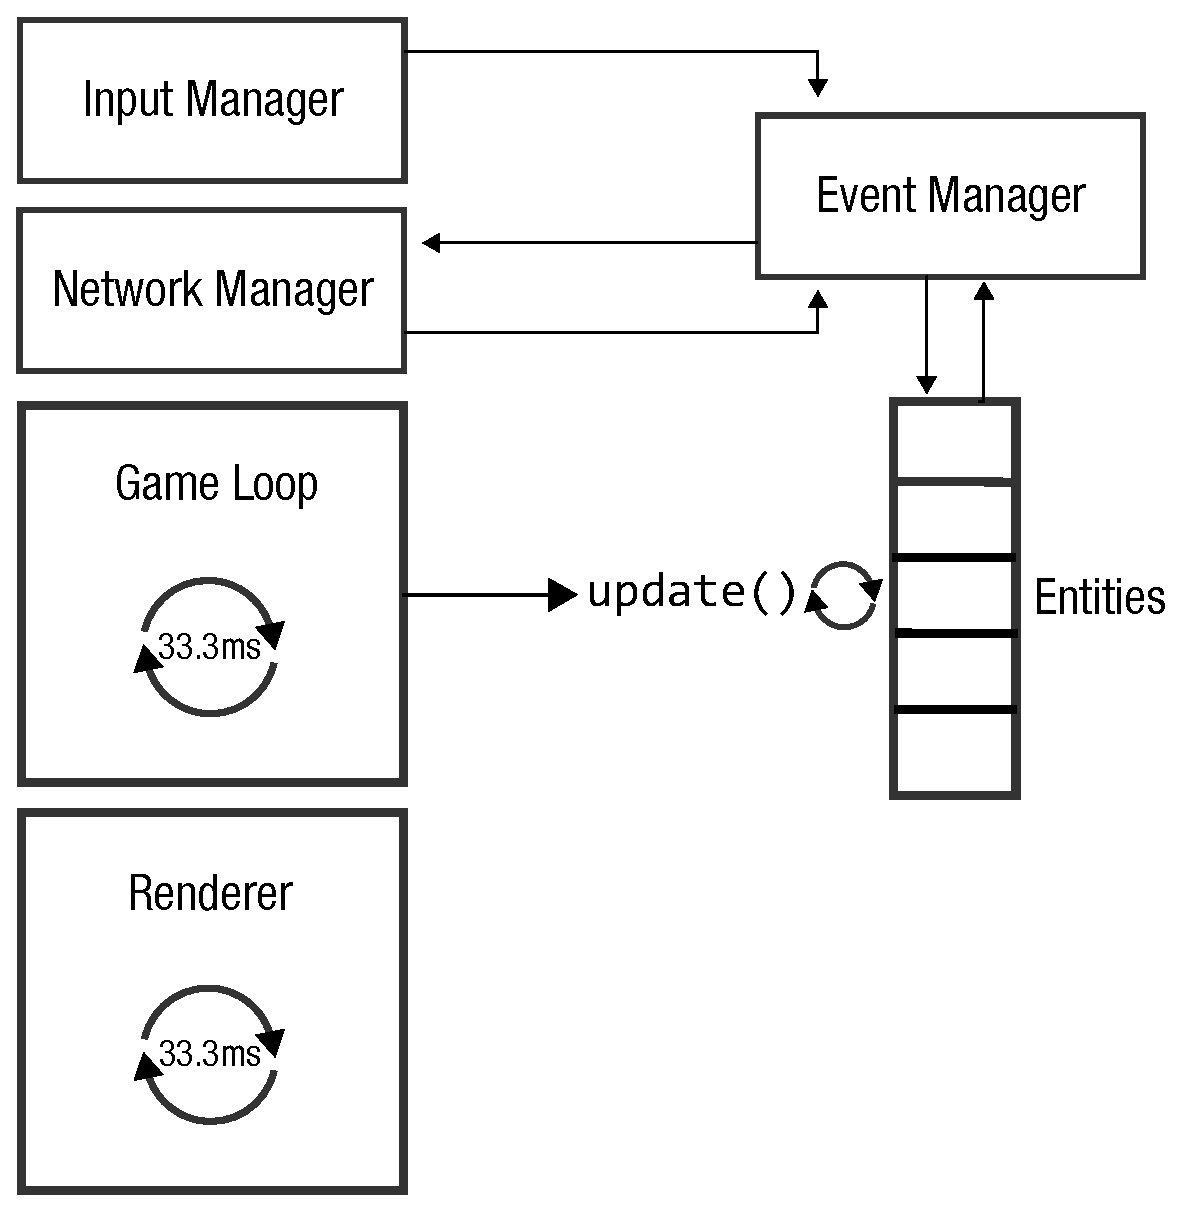
\includegraphics[width=8cm]{Images/overall_architecture.eps}
	\caption{The overall architecture of the game engine.}
    \label{fig:architecture}
\end{figure}

The most important component in the engine is the game loop. This is responsible for the updating of the game simulation every frame by asking each entity it knows about to update itself in turn. When asked to update themselves, the entities check their event queues for any new events and process them as required, then proceed to perform any necessary updates to their state, such as movement, as well as creating their own event to inform the server if relevant. These events are passed around the system by an event manager, which sits outside of the game loop. Any part of the system that wants to know about something registers itself to receive event updates related to that thing and is then given them the moment the event comes in. Finally, there is an input manager and a network manager, which handle input (and output in the case of the network manager) from players and the server.

This architecture applies fully to the client but the server makes some changes. These changes come about primarily due to implementation details and the differences between JavaScript and Python. However, the biggest difference by purposeful design is that the server needs to handle multiple games running simultaneously but apart, rather than having to deal with only one. This means that the server has a higher level manager responsible for creating games and routing messages to and from the server-side games and the clients.

% TODO: DIAGRAMS

\section{Detailed Design}

\subsection{\texttt{Engine} and \texttt{Scene}}
The \texttt{Engine} class is the central class in the game. It manages the creation of all other system classes, including the event manager, the network and input managers and the renderer, and contains the central game loop. Once the game is loaded it tells the server that the client is ready so that it can be registered to receive network events. It is also responsible for creating and giving access to the \textsc{html5} canvas used to render the game.

The \texttt{Scene} class is what describes the actual content of the game simulation at that moment. Each scene represents the map the players are currently on, and contains the terrain as well as all the entities. When the game simulation is updated, it is the entities in the \texttt{Scene} class that are affected.

To load the scene from the server, the \texttt{Scene} class contains several methods that first communicate with the server and then handle the result. The server keeps track of which scene is the currently active one in a game, so \texttt{Scene} gives the server its game ID and is given back the scene data in response. This data is processed and turned into actual terrain and entities. No other part of the game is able to create new entities.

The \texttt{Scene} class also remains the only place where the new event manager was not implemented. Due to the issues with the previous event management system, discussed in section \ref{subsection:eventmanager}, network connectivity had to be implemented directly into \texttt{Scene}, rather than abstracted to the correct \texttt{Network} class. With the event manager, this shouldn't be necessary, but the retrofitting work was not completed in this case.

\subsection{Game Loop}

\begin{figure}[H]
	\centering
	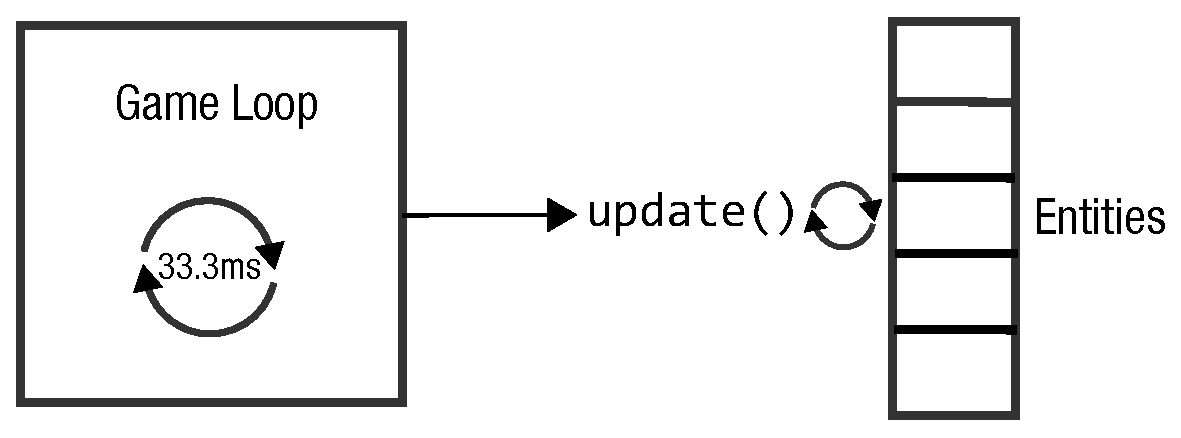
\includegraphics[width=8cm]{Images/game_loop.eps}
	\caption{The game loop updating.}
    \label{fig:gameloop}
\end{figure}

The central part of any game is what is known as the game loop. It is run from the main \texttt{Engine} class and is responsible for managing the entirety of the game, making sure every other part of it runs when it is supposed to.

An important concept to understanding the purpose of the game loop is the \textbf{frame.} This is a slice of time in the game world, with the amount of time each frame represents being decided by how many frames you wish to have per second. Common numbers chosen here are 30 and 60, meaning a frame is 33.3 milliseconds and 16.7 milliseconds respectively. While it is usually trivial to have a simple game running at 60 frames per second, it isn't always the right choice. More frames per second means more processor time used, which drains more power or could cause issues on weak devices. For this project it is also unnecessary, as the game world does not require a simulation at that level of fidelity. 30 frames per second was chosen as a good balance between smoothness of gameplay (such as moving around) and demands on power.

The purpose of the game loop is to update the simulation every frame while keeping track of whether the simulation is running at the correct speed. Every time it runs it first needs to check how much time has passed since the last frame was processed. If, for some reason, a frame took too long to process the last time then the next update will run as many times as necessary to catch back up to where it should be, regardless of whether that means things are moving too quickly in real-time or not.

The game loop itself is not directly responsible for updating the simulation, however. Rather, it calls every entity that is currently active and asks it to update itself. Once all entities have updated themselves, the network manager is asked to inform the server of everything that happened it might need to know about and the frame is complete.

\subsection{Entities}\label{entities_design}
Entities are the next most important part of the game architecture, alongside the event manager, which will be discussed next. Each entity is an object in the game world. In the Component-Entity System mentioned previously, it would be made up of many individual components, linked to a component manager so that they could talk to each other and share necessary state. The entity itself would have no real idea about what it is or what it does, simply getting each component to do something in turn, in a way similar to the game loop asking the entity to update in the first place.

However, because implementing this is very complicated, entities in the project game don't work this way. Instead, they are more traditional objects, with methods and properties. This works fine because there are only two types of entity in the game: a basic \texttt{Entity} and a \texttt{Character}.

The basic \texttt{Entity} class is a simple object in the game world like a wall. It has no properties beyond its size, position and the sprite that represents it if one exists. A \texttt{Character} is a lot more complicated, and has methods for handling user input and updating its position, as well as dealing with any other interactions that might occur, such as taking damage from another entity.

When an entity is asked to update itself, it checks the list of events that it has received from the event manager since the last update and runs through them, applying a series of functions in order. Once it is done the game loop asks the next entity along to do the same thing. Basic entities don't do anything on an update, whereas \texttt{Character}s will check for input from a player or the server and update their positions or perform an action.

The existence of two types of player with different capabilities created some issues. Initially there was actually a third entity type that inherited from \texttt{Character}, called \texttt{Player}. The \texttt{Player} class had extra functionality to find paths for itself, and interpreted player input but not server input. However, because a Game Master needs to be able to change which entity they are controlling, the \texttt{Player} class was merged with \texttt{Character} and a method for swapping between them was created.

As there were two ways to interpret any input events, and they needed to be switched out, two functions were made into components: input handling and path finding. The input handler for an active player listens for events from the input manager, whereas the input handler for a remote player listens for network events. The pathfinding component on an active player actually creates paths, whereas the remote entities simply get given them from the network.

\subsection{Event Manager}\label{subsection:eventmanager}

\begin{figure}[H]
	\centering
	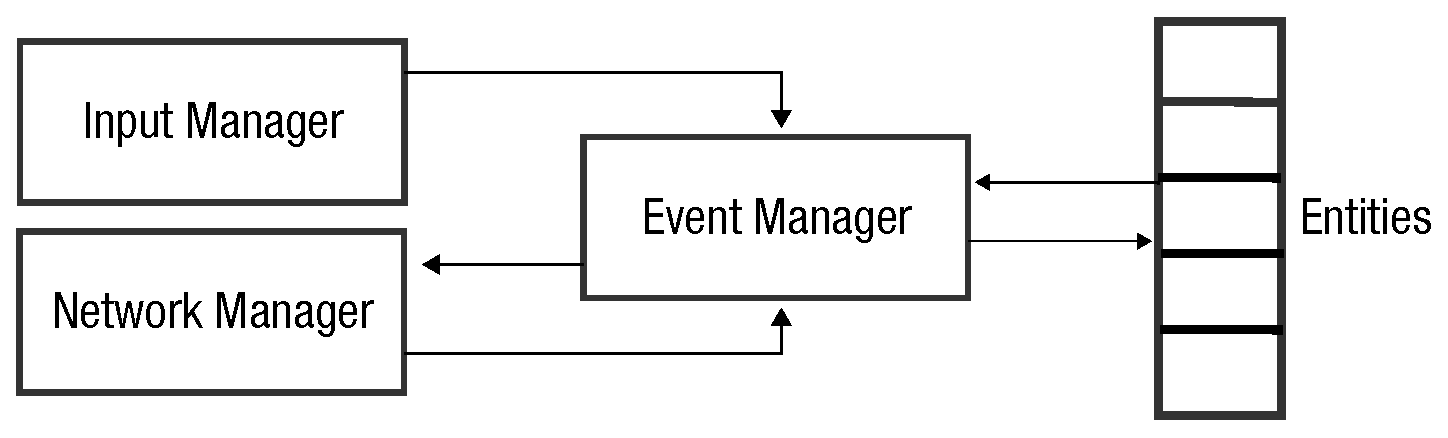
\includegraphics[width=8cm]{Images/event_manager.eps}
	\caption{The event manager.}
    \label{fig:event_manager}
\end{figure}

The event manager is an important piece of the game engine, and is the communication method for all the other system components, acting as a sort of glue between them.

Unlike almost all the other parts of the game, the event manager is not run per frame or controlled by the game loop. Rather, it receives and propagates events as it gets them. This means that events that are created in the middle of a frame's update are still sent to the things that need them.

This has some advantages. The main advantage is network latency. Because the network latency is several frames long, the ability to have the network send events back in the same frame that they happen helps to reduce any time wasted. Another small time-saver in this regard is that an entity affecting another entity may be able to have that effect be known about in the same frame, as long as the acting entity is processed before the entity being acted upon. In the case of an affected entity being updated first, however, it will only take into account the new information in the next frame. This isn't a huge issue, and a user should never really notice that something has happened one frame after, but the inconsistency is there and could potentially cause problems in situations where frames are taking a long time to process.

Despite the seeming obviousness of its use, the event manager originally didn't exist, and input was handled by having a single event queue stored in the \texttt{Engine} class. This event queue was given to entities from the update call in the game loop and they ran over each event looking for something relevant to them. It was also very difficult for entities to put anything into the event queue themselves, such as network input. Because of this, network events were created directly. Worst of all, because there was no way to know whether events were handled, the entire event queue was cleared on each frame, which meant that no events could be carried over.

Obviously this approach had several disadvantages. Firstly it was inefficient. Although generally there was only going to be one or two events in any given frame, there are potentially a lot of entities that have no interest in events that are stored in the event queue, so having them loop over those events is useless. Secondly, in order to update the network or add anything back into the event queue, entities had to be given the network and engine objects and pass them around. The emptying of the entire queue also meant that in situations where one entity wanted to affect another but was updated after the entity it was affecting, the affected entity would never know about it.

Replacing this system with a proper global event manager allowed for entities to no longer care about events that don't matter to them, as well as much more easily carry over events from frame to frame, even leaving events unhandled for a long time if necessary. Unfortunately the refactoring to use the event manager wasn't entirely completed, as seen with the previously mentioned \texttt{Scene} class. However, the vast majority of the game uses it.

\subsection{Renderer}\label{design_renderer}
The renderer is responsible for displaying frames to the player, acting as the view into the simulation. It is also another part of the game engine that is separated from the game loop. It isn't required for this to be the case in order for the game to function; indeed, with the simplicity of the game in this project the renderer could be tied to the game loop's frames pretty easily and cause no problems. It is, however, considered to be good practice to separate them, and for good reason. The renderer is almost always the most taxing part of the whole game. By adding the renderer to the central game loop's update process you cause each frame in the simulation to take a lot longer to complete. If this addition doesn't cause the frame to run over time then no problems will be noticed. Unfortunately, it is very easy for the renderer to cause frames to run over time and, if it happens consistently, the game loop could get stuck in an infinite loop attempting to catch up.

By separating the renderer out, you can make sure that the central game loop always updates correctly and keep the simulation running, regardless of how many frames the renderer is managing to actually display to the user. It is desirable to make sure that the renderer is managing to display all the frames, but it's less of a problem if the renderer can only display 20 of them than it is to have the central game loop stuck trying to catch up.

The renderer does not render the world in one go. Rather, it renders the terrain first, and then renders entities on top of it. The reason for this is one of efficiency. The terrain never moves and never crosses tile boundaries. It also comes pre-ordered in a grid. These attributes make it easy to render by simply drawing each tile to the screen one by one in order. Entities, however, can have different heights and can move around and cross tile boundaries, which requires that they get sorted properly, creating rendering overhead. By rendering the terrain first, there is less that needs sorting afterwards, thus speeding up the renderer.

\subsection{Input Manager}
A game isn't much of a game if the user cannot create any input. To handle the user's input there is an input manager, which is responsible for capturing all of a player's input, working out what purpose that input has and then creating an event for it in the event manager, which propagates it to all interested parties.

The input manager is only able to work out what user input means, not what that input applies to. In other words, it knows that a user clicking means the user wants to move somewhere, checks that it is a valid input and then creates an event to say that there has been a movement input and the tile to move to. This event is passed to all entities that subscribe to movement events and it is up to them to work out whether it is relevant or not.

\subsection{Network}
The \texttt{Network} class is responsible for managing the connection the game has to the server. At the end of every frame it will inform the server of anything the client's player has done, such as moved his character to a new location.

If the server sends a message, however, the network manager will immediately create an event for it. Although this is mostly due to technical implementation reasons, there are advantages in this. Primarily, it means that entities being affected by network events can be updated sooner as they don't necessarily have to wait till the next frame. This is important for the same reason as the event manager, by reducing latency from a very high latency aspect of the game.

\subsection{Server Differences}
%todo: add diagrams here explaining the server architecture

\begin{figure}[H]
	\centering
	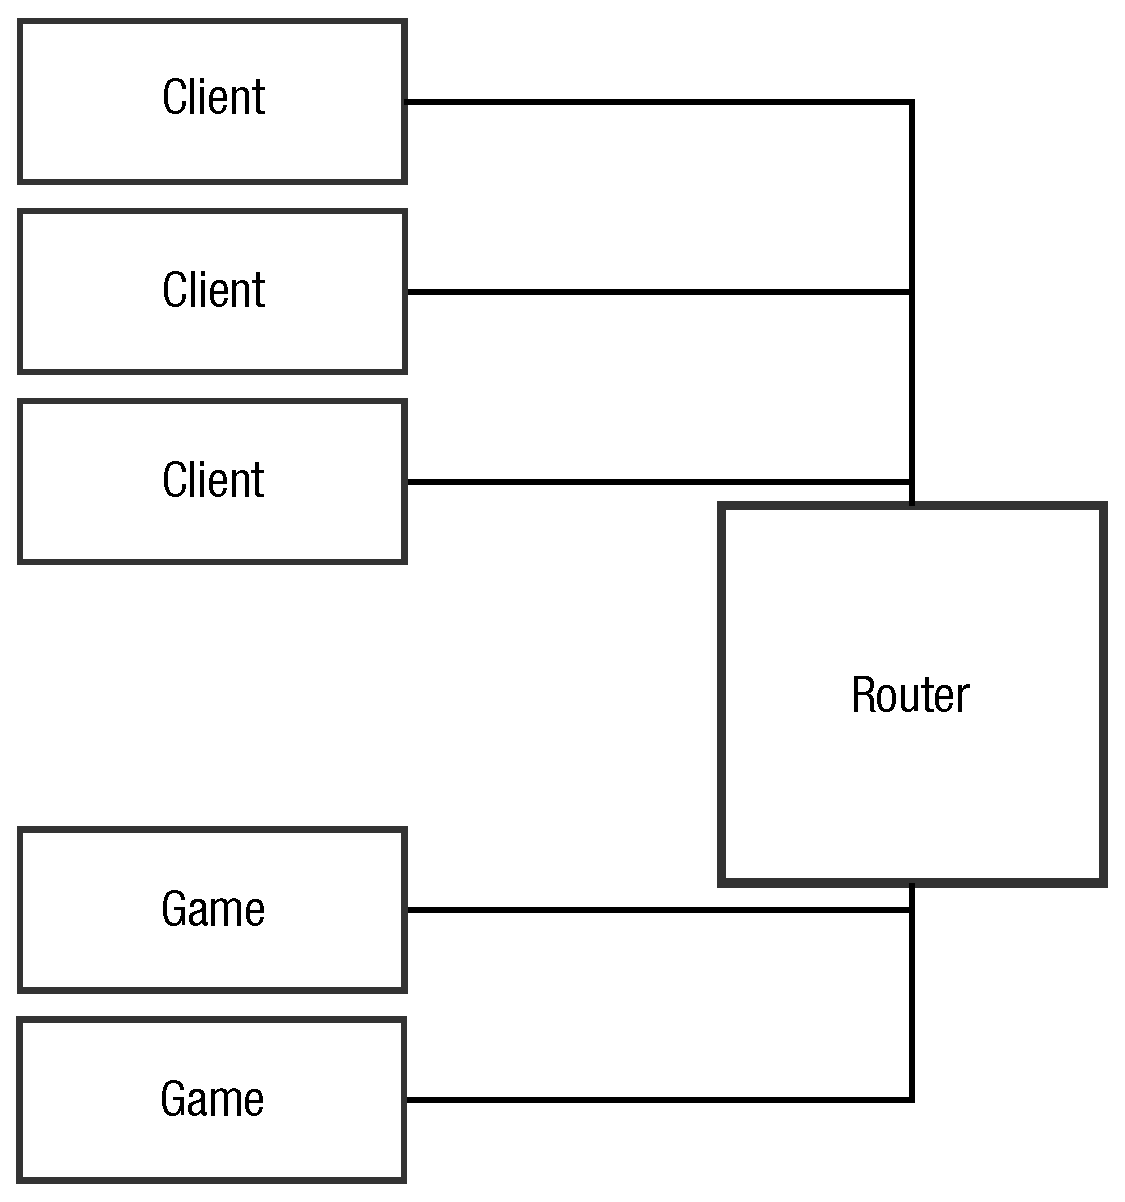
\includegraphics[width=8cm]{Images/server_design.eps}
	\caption{The server contains the router and some games. The clients interact with the game they are interested in through the router.}
    \label{fig:server_design}
\end{figure}


The server's purpose is to act as a central version of the game that links all the clients together, and is responsible for being something of an authority in the game simulation to make sure that clients see the correct things. Because of this it makes sense that the server and client have the same structure.

However, there are, in fact, differences between them. The reason for this is entirely due to implementation---which will be discussed in more detail in the next chapter---but regardless of the reasons it's important to understand these differences.

The most important and major difference is that the server runs many games simultaneously, rather than just a single game at a time. To handle this, a higher level is needed to manage the games and route messages to and from players. The router that handles this is a traditional web application router, made using the Flask framework. It takes incoming HTTP connections and works out what they are supposed to do based on the URL. Once a game is up and running and users are connected, they communicate with it through the SocketIO library providing websockets, which the router also manages.

Each game itself is run in a separate thread, providing an architecture as similar to the one in the client as possible. Communication between the router and any individual game is handled through thread-safe queues, as it is impossible to call a method in the thread directly due to the game loop blocking and taking control.

The game loop itself is probably the most major difference in the internal game architecture, entirely by way of implementation details. The client's JavaScript version of the game loop is essentially non-blocking as it has to always yield control back to the browser. However, Python has no native way of achieving this style---known as an event loop---and the libraries available to implement it are complicated. Because of this, the Python implementation of the game loop is a more traditional \texttt{while} loop, running until a flag indicating the game is to be shut down is set to false.

Although this does not affect the fundamental way of updating entities, which is the bulk of the work the game simulation performs on the server, other aspects of the architecture are changed because of it.

There is no proper event manager in the style that was added to the client, as there is no easy way for it to be run outside of the game loop without creating another separate thread for it---an undesirable option for a server that will already be having to manage many of them. Because of this, the server event management remains in the original style that the client had before the event manager was implemented: the game loop contains a data structure that stores all the events and asks the entities to take a look at them in turn and see whether they care.

In a concession to sanity, however, the server uses a queue to store input events (accessible by the router so that they can be passed in) and doesn't delete unhandled events at the end of every frame. Output is placed into another queue that the router can check in order to inform clients of anything interesting.

Other parts of the architecture are simply removed: there is no renderer because the server's view is entirely remote---no one is ever going to be trying to play the game on the server directly. The server also doesn't have an input manager for the same reason. The network manager is pushed up into the router, rather than being a special part of the game engine.

This design is, of course, not perfect. The biggest issue is one of scalability. This model works fine for one or two games running at once, but because the router has to manage connections for all active games it can very quickly get overloaded, especially when players decide to spam actions that create network events such as movement commands.

Ideally each game would be responsible for handling its own connections and the router would simply exist to get players connected to the right game. This creates independence of the router and game servers and is a much more scalable solution. The reason it doesn't do this, however, is just because the implementation knowledge necessary for this was not available and time did not allow for further investigation into it. A less than ideal working solution was considered to be the better choice than potentially having no solution at all because the implementation was too hard given skill, knowledge and time available.

% The game simulation running on the server operates with the same fundamental architecture, with the exception of having no input manager as there can never be any direct input to the server. However, because the server has to operate many games at once, there is another level higher than the client-side has.

% The server has a traditional web application router that receives and routes events from the client. These events are things like joining or leaving a game as well as the things a client cares about like movement. In this way, it takes the place of the \texttt{Network} class in the client.

% Each individual game is run in a separate thread due to the blocking nature of the game loop. The server keeps track of who is connected to what game and sends events that are relevant to a game to that game alone, which means that there is no pointless spamming of irrelevant events to games that don't care about it.

% This higher level part of the server is also responsible for creating game threads when a user first connects to a game. However, the game loop itself is responsible for shutting itself down, though the router can ask the game to do so as well.

% You should concentrate on the more important aspects of the design. It is essential that an overview is presented before going into detail. As well as describing the design adopted it must also explain what other designs were considered and why they were rejected.

% The design should describe what you expected to do, and might also explain areas that you had to revise after some investigation.

% Typically, for an object-oriented design, the discussion will focus on the choice of objects and classes and the allocation of methods to classes. The use made of reusable components should be described and their source referenced. Particularly important decisions concerning data structures usually affect the architecture of a system and so should be described here.

% How much material you include on detailed design and implementation will depend very much on the nature of the project. It should not be padded out. Think about the significant aspects of your system. For example, describe the design of the user interface if it is a critical aspect of your system, or provide detail about methods and data structures that are not trivial. Do not spend time on long lists of trivial items and repetitive descriptions. If in doubt about what is appropriate, speak to your supervisor.

% You should also identify any support tools that you used. You should discuss your choice of implementation tools - programming language, compilers, database management system, program development environment, etc.

% Some example sub-sections may be as follows, but the specific sections are for you to define.

% \section{Overall Architecture}

% \section{Some detailed design}

% \subsection{Even more detail}

% \section{User Interface}

% \section{Other relevant sections}
\chapter{Implementation}

INTRODUCTION GOES HERE

\section{Renderer}
The graphics renderer was the first piece of the game engine worked on. Having the graphics to provide a view into the game world was important in order to easily see whether things were behaving as expected and proved extremely useful in detecting problems with other parts of the game later on.

This section will go over firstly what isometric projection is and then the ways that graphics are actually drawn to the screen. Finally, the difficulties that the renderer caused during implementation will be discussed.

\subsection{Isometric Tiles}

\subsubsection{What Is Isometric?}
When talking about isometric projection in the videogame world it is important to know that it is not truly isometric. True isometric is an ``axonometric projection in which the three coordinate axes appear equally foreshortened and the angles between any two of them are 120 degrees'' \todo{reference}. What the gaming world calls `isometric' is in fact \textit{dimetric} projection \todo{reference}---a projection where two axes are the same but the third is not.

The reasons for doing this are essentially one of aesthetics when drawing objects at a very low resolution with visible pixels. At these very coarse resolutions, true isometric projection creates an aesthetically displeasing line. However, by changing to a dimetric projection, where the line grows twice as fast horizontally as it does vertically, the line becomes much more consistent and visually appealing. \todo{figure}

\subsubsection{Cartesian To Isometric}
The term ``\textsc{2d} isometric tile'' used in this report is a little ambiguous. The game world itself is represented by simple \textsc{2d} Cartesian coordinates that map to a grid of tiles. Isometric space, however, is \textsc{3d}. The term used here refers to the type of graphic used to represent the tiles in isometric space, rather than the isometric space itself. These graphics are simple \textsc{2d} images, drawn in such a way as to make them look \textsc{3d}. \todo{figure showing cartesian and isometric}

Of course, this means that a conversion has to be made between the two coordinate systems in order for the renderer to be able to display things in their proper place. As an example, figure \todo{figure} shows what the game world looks like if it is rendered without this coordinate conversion---clearly very wrong.

In order for the renderer to show things correctly in the isometric space there needs to be a way of converting between the game world's Cartesian coordinates and the renderer's isometric coordinates. Luckily, this is incredibly simple:

\noindent
\begin{minipage}{\linewidth}
\begin{lstlisting}[style=js, caption={JavaScript implementation of a function to turn Cartesian coordinates into game isometric coordinates. Original algorithm from \cite{citeulike:13155325}.}, label=cartesian_to_isometric]
function cartesianToIsometric(cartesian_x, cartesian_y)
{
	var isometric = {};

    isometric.x = cartesian_x - cartesian_y;
    isometric.y = (cartesian_x + cartesian_y) / 2;

    return isometric;
}
\end{lstlisting}
\end{minipage}

Now when the renderer draws the game to the \textsc{html5} canvas, it can first call the \texttt{cartesianToIsometric} function, letting it place the tile graphics in the correct place as seen in figure \todo{figure}.

\subsection{Rendering}
After the renderer has converted between Cartesian and isometric spaces it needs to be able to draw things to the canvas. The actual drawing of a game tile to the canvas is straightforward, simply requiring a call to the canvas's \texttt{drawImage()} function and supplying it the image you wish to draw and the canvas coordinates for where you wish it to be drawn.

The difficult part comes before that. Firstly, you need to be able to work out what the canvas coordinates are. The conversion between isometric coordinates and the canvas coordinates works as follows:

\noindent
\begin{minipage}{\linewidth}
\begin{lstlisting}[style=js, caption={Conversion between isometric coordinates and canvas coordinates.}, label=isometric_to_canvas]
canvas_x = isoCoords.x * (TILE_WIDTH / 2);
canvas_y = isoCoords.y * (TILE_HEIGHT / 2) - (image_height - (TILE_HEIGHT / 2));
\end{lstlisting}
\end{minipage}

A few things should be explained about this. Firstly, \texttt{TILE\_WIDTH} and \texttt{TILE\_HEIGHT} refer to the set size of a single tile and are used to work out the tile's positioning in the world. The \texttt{image\_height} value refers to how tall in pixels an image is. Theoretically an image can have any size and isn't limited to how large a tile is. However, in practical terms, an image can only be arbitrarily tall; width needs to be kept within the tile limits or there will be problems with depth sorting, for reasons seen in section \ref{entity_rendering}.

\todo{a figure showing the difference between a tile and the image representing it}

Also worth noting is that there are separate rendering functions used for the terrain and the entities. The terrain has no height value, but even if it did it is rendered in such a way as to make it irrelevant, so the drawing of terrain tiles excludes the \texttt{image\_height} part of the calculation.

Once you have the coordinates you then need to get the tile graphic to use as the image being rendered. Getting the image itself is a very simple task, but getting the order in which to draw them right is more difficult.

The \textsc{html5} canvas is a very simple element and it has no ability to specify the relative depth of things being drawn to it; whatever is drawn first will be occluded by what comes afterwards if they overlap. This overlapping is often not a problem when drawing simple \textsc{2d} tiles with a top-down or side-on perspective. However, because the isometric perspective is \textsc{3d} the issue of depth becomes an important one.

\todo{Figure of what it looks like when depth sorting is broken}

There are two methods for solving this used in the renderer: a simple painter's algorithm and a depth sorting algorithm. The first is used for the terrain and the second for entities.

\subsubsection{Terrain Rendering}
The terrain is very simple to render as far as isometric projection goes. Terrain images are the same size as the tiles, which means that as long as they are drawn in order the images will never overlap.

The method for achieving this ordering is known as a painter's algorithm\footnote{The painter's algorithm is so called because of a common painting technique whereby distant parts are painted before closer parts that might cover them.} and is very simple. Firstly, all the terrain is stored in a pre-sorted, two dimensional array. Columns are labelled \texttt{y} and rows are labelled \texttt{x}. Images are drawn by looping through each row in each column and drawing them one by one, rendering the images from back to front, row by row.

\todo{Diagram showing how the painter's algorithm works}

This is a very efficient and cheap way to render the images to the screen, and works perfectly for the terrain. Even if the terrain were to be made no longer flat, as long as it never broke out of the tile grid there would be no need to change how it is rendered.

\subsubsection{Entity Rendering}\label{entity_rendering}
Unfortunately, entities are less easy to deal with. At least some entities can move around---crossing tile boundaries when they do so---which means they cannot be stored in the same grid that makes up the tiles themselves. Because entities can exist outside of the tile boundaries, working out their depth cannot be done just by iterating through them like the terrain. Another way has to be devised in order to render them in the correct order.

To figure out the order that entities need to be rendered it is first necessary to work out what their relative depth in the scene is. To get an entity's depth, the following calculation is used:

\noindent
\begin{minipage}{\linewidth}
\begin{lstlisting}[style=js, caption={Calculation to work out an entity's relative depth in the scene.}, label=calculate_depth]
function calculateDepth(entity) {
    return Math.round((entity.x * TILE_WIDTH / 2) + (entity.y * TILE_HEIGHT / 2) + entity.z);
}
\end{lstlisting}
\end{minipage}

In this calculation, the most important part is the addition of an entity's position data, \texttt{x}, \texttt{y} and \texttt{z}. The \texttt{z} attribute is not currently used in the game, but if it were it would represent relative height from the ground plane and is thus important to the depth calculation. The use of the \texttt{TILE\_HEIGHT} and \texttt{TILE\_WIDTH} attributes is due to the small values of the position data. Because tiles can potentially have small values like \texttt{(1, 1)}---though they could also in theory be very large---it is often common for depth values to be worked out as being the same. Multiple entities sharing a depth value will often cause them to be rendered in the wrong order. The other issue is that positions can be non-integer, such as \texttt{(1.250, 1)}. The sorting method used can't handle this, so it's necessary to round to a whole number in order to make sure it doesn't break.

The sorting method itself is a modified pigeonhole sort, as shown in Listing \ref{depth_sort}.

\noindent
\begin{minipage}{\linewidth}
\begin{lstlisting}[style=js, caption={Depth sorting entities in a scene using a modified pigeonhole sort.}, label=depth_sort]
function depthSort(entities) {
    var buckets = [];

    for (entity in entities) {
        var depth = this.calculateDepth(entities[entity]);

        if (!buckets[depth])
            buckets[depth] = [];
        buckets[depth].push(entities[entity]);
    }

    var result = [];

    for (bucket in buckets) {
        for (entity in buckets[bucket]) {
            result.push(buckets[bucket][entity]);
        }
    }

    return result;
}
\end{lstlisting}
\end{minipage}

The pigeonhole sort works well for this task. The first reason for this is that the number of entities and number of keys are almost always the same, and even when not the smaller number of keys does not affect the performance of the sort. The number of entities being placed into the sort is also usually very small, which means that memory is not a concern, though with a very large number of entities the memory footprint could be a problem. The other reason the pigeonhole sort works well is that it keeps intact the link between a depth value and the entity it represents without any extra work. This means that the sorted array containing the entities can be used directly in the renderer, saving development and processor time.

The sorted array that comes out of the pigeonhole sort is flat, so the renderer only needs to loop through it once in order to render all the entities to the canvas at the correct depth.

\subsubsection{Depth Sorting Limitations}
The depth sorting used in the project works well and performs as expected. However, it has a major limitation in that it will not work for entities that can exist across multiple tiles. Currently, all entities are the size of a single tile---though they may have arbitrary height within it. This makes calculating the depth a simple case of looking at position. If an entity were to be larger than a single tile, however, the position data would not be sufficient to determine depth.

There are two ways to have entities that can exist across multiple tiles. The first is to have the entities be actually made up of multiple tiles. There are two frustrations with this. The first is that artwork needs to be split up into multiple tiles, which means that content in the game is harder to create. The second is that entities need to keep track of what tiles they are taking up, creating further work for the sorting algorithm to do in order to figure out what is where and gaining little over simply having lots of separate entities pushed together to appear whole.

The better option here is to keep a model of an entity's position in \textsc{3d} space. Although the entities themselves are rendered with \textsc{2d} images, because of the isometric projection they still exist in \textsc{3d} space. By keeping data that models this three dimensionality it is possible to work out the depth of an entity without associating it with more than one tile. Instead, it is given a central tile and the data about its size fills out the rest of it.

This approach affects more than just the rendering. By having an actual size in \textsc{3d} space entities can be interacted with in a more fine-grained way. For example, the current system of collision detection simply checks to see whether a tile position contains an entity or not. This is relatively simple to implement but it is not very versatile---position data is very coarse. By turning the game world into a \textsc{3d} simulation it is suddenly possible for position data to be more fine-grained. Not only can the renderer work out the depth of something that is not bound by whole tiles, collision detection is no longer bound by whole tiles either.

Of course, doing this is very complicated and would require a complete rewrite of almost all of the game engine's underlying systems. Given the difficulties already encountered when implementing what was there it was decided that the huge effort involved was not worth it.

\subsection{Renderer Implementation Difficulties}
Being the first major feature to be worked on meant that the renderer was subject to a lot of change and iteration as the project developed. Things that appeared to be working fine at first turned out to be inadequate when other features were added. The renderer was probably the most rewritten and refactored part of the entire code base.

The terrain has been the most stable part, with the rendering method being unchanged since it was first implemented. However, the entity rendering was changed a great deal. The initial implementation had the entities rendered in a way similar to the terrain, by placing them into an array at the correct locations and then iterating through it. While this technically worked, it was ugly and was soon found to be completely inadequate once entity movement was introduced to the game.

The method for rendering entities including the depth sorting also did not work perfectly the first time either. At first the pigeonhole sort was not working properly, as entities were overwriting each other when they had the same depth value. This was solved by introducing the idea of buckets that could store multiple entities at once when they had the same depth value. The next step to solving this was to make sure that the depth values weren't so small. The depth values being taken only from the very small tile positions was causing them to often have the same depth value and unable to be sorted correctly as too many of them were being put into a bucket together. This was solved by adding the tile values to the calculation, which created much more variation in depth. It is now far rarer for entities to share a depth value, and when they do they do not overwrite each other.

Beyond these specific problems, the renderer's place as first feature implemented also suffered from the lack of experience, in JavaScript, use of the \textsc{html5} canvas and games programming in general. A lot of time was spent researching and iterating on things that now would be much easier to implement and be done in a lot shorter time.

\section{Input and Movement}
Movement is one of the most important user facing features of the project. It also makes use of several parts of the game engine to work properly, relying on the game loop functioning correctly to advance the entity at the correct pace, the renderer to display this movement across tiles correctly and both the input manager and network manager to receive (and send) commands.

\subsection{Input}
The first and most important of these major parts is the input handler. Originally, the input handler was contained entirely in the \texttt{Engine} class. However, with the advent of the event manager it was refactored out into its own class.

Input in the game is mouse-based, rather than keyboard-based. Being mouse-based, input is a little more difficult to handle than if it were possible to simply capture a button press. It is necessary to work out what location exactly the player has clicked, then go through a series of functions to turn the click location into game-world coordinates. Once the coordinates are known, they need to be checked for validity and then passed on, along with the event type, to any entities that might care to know about it.

The first step in this is capturing the user's input. Browsers are helpful in that they keep track of where the user has clicked, which means that the browser event can be captured and used for the game's purposes. To listen for user clicks, a click event listener is attached to the game's canvas. Unfortunately, however, despite being attached to the canvas, the click event coordinates are global to the window, rather than being constrained by the canvas. What this means is that click coordinate \texttt{(0,0)} is not, in fact, the corner of the canvas, but instead the corner of the browser window that contains the canvas.

To solve this, it is necessary to work out the click's position relative to the canvas. This is accomplished using the code in listing \ref{canvas_click_coordinates}.

\noindent
\begin{minipage}{\linewidth}
\begin{lstlisting}[style=js, caption={Transforming a user's click to be relative to the canvas, rather than the window.}, label=canvas_click_coordinates]
canvasPosition.x = ((event.clientX - this.engine.camera.x) - this.engine.canvas.offsetLeft) - (TILE_WIDTH / 2);
canvasPosition.y = ((event.clientY - this.engine.camera.y) - this.engine.canvas.offsetTop);
\end{lstlisting}
\end{minipage}

There are a few things to note in this code. First of all, the \texttt{event} used here is the one passed in from the click event listener, and is an object supplied by the browser. The next thing to note is the \texttt{camera} object. This is a game object that acts as the user's viewport into the world. Because the world can be bigger than the canvas itself, it is necessary to have a method of moving the view around the world, which is where the camera comes in. The camera object has an offset, which the renderer takes into account when positioning entities onto the canvas. Of course, this offset needs to be taken into account when detecting where, exactly, the user has clicked in the world, and so it is used here to do that. The coordinates are then set to be relative to the canvas instead of the window by using the \texttt{offsetLeft} and \texttt{offsetTop} values on the canvas itself, which refer to the canvas' position in the browser window.

After this, a set of functions are used to first transform the canvas' isometric coordinates into \textsc{2d} Cartesian coordinates, and then from there to turn those into actual tiles, shown in Listing \ref{iso_cart_tile_coords}.

\noindent
\begin{minipage}{\linewidth}
\begin{lstlisting}[style=js, caption={Turning the canvas isometric coordinates into \textsc{2d} Cartesian coordinates and then into tile positions. Original algorithm to transform isometric to Cartesian space from \cite{citeulike:13155325}.}, label=iso_cart_tile_coords]
var cartCoords = (function(x, y){
    var coords = {};
    coords.x = (2 * y + x) / 2;
    coords.y = (2 * y - x) / 2;
    return coords;
})(canvasPosition.x, canvasPosition.y);

var tileCoords = (function(x, y){
    var coords = {};
    coords.x = Math.floor(x / (TILE_WIDTH / 2));
    coords.y = Math.floor(y / (TILE_WIDTH  / 2));
    return coords;
})(cartCoords.x, cartCoords.y);
\end{lstlisting}
\end{minipage}

With the tile coordinates acquired, they are sent into a method to work out what to do with them. It first checks for the validity of the tile coordinate by checking whether it is inside the bounds of the map. Assuming the coordinates are in bounds, a check is then done to see whether the player has clicked on an entity or whether they have clicked on a terrain tile. Clicking on an entity could mean either an invalid click location or a command to change to controlling that entity, depending on whether the user is the Game Master or not. However, clicking on a blank tile---and thus the terrain---always means a movement command.

\subsection{Movement}
There are two methods of giving an entity a movement command. The first is from the direct input as detailed in the previous section. The other is input from the network. These work similarly but not entirely the same.

When handling input, all moveable entities are subscribed to events for both direct input and network input. Whether they do something with the direct or network input depends on the component they are using to handle it. For a player character, the direct input event is handled. For a remote character the network event is handled instead.

\subsubsection{Direct Input}
With the event processed, a series of other methods are called to move the entity. The first step is the pathing step, which makes use of the other changeable component in the \texttt{Character} class. For direct input, the entity needs to figure out the path it is going to take to move from its current position to the newly selected one. The first step here is to check whether or not the entity is currently following a path. If it is following a path then its location may not be a whole tile, which would cause the pathfinding algorithm to break. In cases where the entity is already following a path, it's next tile destination is used as the entity location instead of its current location.

The pathfinding algorithm used is a library implementation of A*. This implementation provides what is known as the Manhattan style pathfinding, which does not allow diagonal movement. Although this is not the most efficient form of pathfinding, it was decided as being the best option for a variety of reasons. The first of these reasons is one of gameplay. With the tile-based nature of the game, diagonal movement feels somewhat odd. The second reason is one of artwork; in theory, having 8 directions of movement creates a need for extra animations and graphics for the players---although in reality no animation system was put in, nor were proper character graphics made.

The final reason was to do with collision detection and rendering. Because of the way collision detection works, entities crossing each other diagonally actually end up intersecting with each other, which is an ugly graphical artefact. As was discussed in the previous section on graphics, the work needed to make this a non-issue is considerable and there is little reason to allow for diagonal movement anyway.

The path returned from the A* algorithm is a series of tiles. To follow this path an entity first takes the next tile in the list and sets that as its destination. Whenever it reaches a destination, the path is checked again and a new destination selected. Once the path is completed there are no more destinations to get.

To actually move towards a destination, the entity uses the \texttt{updatePostion} function, which performs a series of checks to determine the entity's current location compared to its destination. When the direction of movement is established, the entity's speed value is added to its position. This speed value is low, being just 0.125, taking eight frames to move an entire tile, though in theory adjusting the speed value would allow an entity to move fast or slower.

Finally, an event is created to inform the server that the entity is going to move and to supply the path it is going to take to get to its destination.

\subsubsection{Network Input}
Movement of an entity that is not under the direct control of the client's player is very similar to moving one controlled through direct input. The difference is that when using network input an entity is given a path, rather than having to find the path for itself.

It is important that a remote controlled entity does not find its own path because it is possible for that path to be different across different clients. Although the short distances available in the test map of the game showed that entities almost always take the same path regardless, in theory it is possible that by simply telling a remote entity to move to somewhere else the entity could end up taking a radically different path. As the game currently stands this isn't the biggest issue in the world. However, in a situation where full interaction with other entities was possible it could prove to be disastrous, as a client may see itself as unable to perform an action on an entity it should be allowed to affect, or vice versa.

Currently, network input is simply taken from the client that created it and echoed by the server. Of course this is not ideal and in theory could produce terrible results due to malicious players. However, difficulties with the server implementation that are discussed in section \ref{server_implementation} will explain why it was done this way.

\subsubsection{Without Input}
Not every frame will have input from a player or the network. Despite this entities are still required to continue their movement. To deal with this each entity stores its current destination and its path as object variables. Every frame the \texttt{updateDestination} and \texttt{updatePostition} functions are called and make use of these variables. Regardless of whether there is input or not these two functions are called, and do nothing if there are no destinations to set or paths to follow.

\section{The Server}\label{server_implementation}


% The implementation should look at any issues you encountered as you tried to implement your design. During the work, you might have found that elements of your design were unnecessary or overly complex; perhaps third party libraries were available that simplified some of the functions that you intended to implement. If things were easier in some areas, then how did you adapt your project to take account of your findings?

% It is more likely that things were more complex than you first thought. In particular, were there any problems or difficulties that you found during implementation that you had to address? Did such problems simply delay you or were they more significant?

% You can conclude this section by reviewing the end of the implementation stage against the planned requirements.
\chapter{Testing}

Detailed descriptions of every test case are definitely not what is required here. What is important is to show that you adopted a sensible strategy that was, in principle, capable of testing the system adequately even if you did not have the time to test the system fully.

Have you tested your system on �real users�? For example, if your system is supposed to solve a problem for a business, then it would be appropriate to present your approach to involve the users in the testing process and to record the results that you obtained. Depending on the level of detail, it is likely that you would put any detailed results in an appendix.

The following sections indicate some areas you might include. Other sections may be more appropriate to your project. 

\section{Overall Approach to Testing}

\section{Automated Testing}

\subsection{Unit Tests}

\subsection{User Interface Testing}

\subsection{Stress Testing}

\subsection{Other types of testing}

\section{Integration Testing}

\section{User Testing}
\chapter{Evaluation}

Examiners expect to find in your dissertation a section addressing such questions as:

\begin{itemize}
   \item Were the requirements correctly identified? 
   \item Were the design decisions correct?
   \item Could a more suitable set of tools have been chosen?
   \item How well did the software meet the needs of those who were expecting to use it?
   \item How well were any other project aims achieved?
   \item If you were starting again, what would you do differently?
\end{itemize}

Such material is regarded as an important part of the dissertation; it should demonstrate that you are capable not only of carrying out a piece of work but also of thinking critically about how you did it and how you might have done it better. This is seen as an important part of an honours degree. 

There will be good things and room for improvement with any project. As you write this section, identify and discuss the parts of the work that went well and also consider ways in which the work could be improved. 

Review the discussion on the Evaluation section from the lectures. A recording is available on Blackboard. 
% add any additional chapters here

\setemptyheader
\addcontentsline{toc}{chapter}{Appendices}
\chapter*{Appendices}
\pagebreak

% start the appendix - sets up different numbering
\fancypagestyle{plain}{%
%\fancyhf{} % clear all header and footer fields
\fancyhead[L]{\textsl{Appendix\ \thechapter}}
\fancyhead[R]{\textsl{\leftmark}}}

\appendix
\fancyhead[L]{\textsl{Appendix\ \thechapter}}
\fancyhead[R]{\textsl{\leftmark}}
\fancyhead[C]{}
\fancyfoot[C]{\thepage}
\renewcommand{\headrulewidth}{0.4pt}
\renewcommand{\chaptermark}[1]{\markboth{#1}{}}

\fancyhead[L]{\textsl{Appendix\ \thechapter}}
\fancyhead[R]{\textsl{\leftmark}}
\fancyfoot[C]{{\thepage} of \pageref{LastPage}}

% include any appendices here
\chapter{Third-Party Code and Libraries}

\section{JavaScript A* Pathfinding Library}\label{pathfinding_library}

This library is used to supply A* pathfinding for movement in the game's client\cite{citeulike:13160393}. The library is released under the MIT License
\cite{MITLicense} and is used with some modification.

\section{Flask Microframework}

This framework supplies the routing and HTML template rendering functionality, as well as the base for other plugins that are used on the server\cite{citeulike:13160396}. It is distributed under the BSD License \cite{FlaskBSDLicense} and is used without modification.

\subsection{Flask-SocketIO}
A plugin for the Flask framework implementing the SocketIO library. It is distributed under the MIT License\cite{MITLicense} and is used without modification.

\subsection{Flask-SQLAlchemy}
A plugin for the Flask framework implementing the Python SQLAlchemy ORM. It is distributed under Flask's BSD License \cite{FlaskBSDLicense} and is used without modification.

\subsection{Flask-WTF}
A plugin for the Flask framework implementing the Python WTForms library for managing web forms. It is distributed under a BSD License \cite{WTFBSDLicense} and is used without modification.

% If you have made use of any third party code or software libraries, i.e. any code that you have not designed and written yourself, then you must include this appendix.

% As has been said in lectures, it is acceptable and likely that you will make use of third-party code and software libraries. The key requirement is that we understand what is your original work and what work is based on that of other people.

% Therefore, you need to clearly state what you have used and where the original material can be found. Also, if you have made any changes to the original versions, you must explain what you have changed.

% As an example, you might include a definition such as:

% Apache POI library � The project has been used to read and write Microsoft Excel files (XLS) as part of the interaction with the client�s existing system for processing data. Version 3.10-FINAL was used. The library is open source and it is available from the Apache Software Foundation
% \cite{apache_poi}. The library is released using the Apache License
% \cite{apache_license}. This library was used without modification.

\chapter{Code samples}

\section{Random Number Generator}

The Bayes Durham Shuffle ensures that the psuedo random numbers used in the simulation are further shuffled, ensuring minimal correlation between subsequent random outputs \cite{NumericalRecipes}.

\begin{verbatim}
 #define IM1 2147483563
 #define IM2 2147483399
 #define AM (1.0/IM1)
 #define IMM1 (IM1-1)
 #define IA1 40014
 #define IA2 40692 
 #define IQ1 53668
 #define IQ2 52774
 #define IR1 12211
 #define IR2 3791
 #define NTAB 32
 #define NDIV (1+IMM1/NTAB)
 #define EPS 1.2e-7
 #define RNMX (1.0 - EPS)
 
 double ran2(long *idum)
 {
   /*---------------------------------------------------*/
   /* Minimum Standard Random Number Generator          */
   /* Taken from Numerical recipies in C                */
   /* Based on Park and Miller with Bays Durham Shuffle */
   /* Coupled Schrage methods for extra periodicity     */
   /* Always call with negative number to initialise    */
   /*---------------------------------------------------*/	
 
   int j;
   long k;
   static long idum2=123456789;
   static long iy=0;
   static long iv[NTAB];
   double temp;
 
   if (*idum <=0)
   {
     if (-(*idum) < 1)
     {
       *idum = 1;
     }else
     {
       *idum = -(*idum);
     }
     idum2=(*idum);
     for (j=NTAB+7;j>=0;j--)
     {
       k = (*idum)/IQ1;
       *idum = IA1 *(*idum-k*IQ1) - IR1*k;
       if (*idum < 0)
       {
         *idum += IM1;
       }
       if (j < NTAB)
       {
         iv[j] = *idum;
       }
     }
     iy = iv[0];	
   }
   k = (*idum)/IQ1;
   *idum = IA1*(*idum-k*IQ1) - IR1*k;
   if (*idum < 0)
   {
     *idum += IM1;
   }
   k = (idum2)/IQ2;
   idum2 = IA2*(idum2-k*IQ2) - IR2*k;
   if (idum2 < 0)
   {
     idum2 += IM2;
   }
   j = iy/NDIV;
   iy=iv[j] - idum2;
   iv[j] = *idum;
   if (iy < 1)
   {
     iy += IMM1;
   }
   if ((temp=AM*iy) > RNMX)
   {
     return RNMX;
   }else
   {
     return temp;	
   }
 }
 
\end{verbatim}


\chapter{Original Proposal}\label{appendix:designspec}

An online, multiplayer roleplaying game similar to \textit{Dungeons \& Dragons} hosted in the browser. The game will have a Game Master and several players in a group. The players move around the world and interact with it and the people/creatures in it and the Game Master guides the players, sets rules and manages the experience. They will be able to manipulate the game world and do things players can't do. For example, they could teleport a player to another location, spawn new monsters or change the weather.

It will include isometric graphics and aim to be as permissive as possible in what players are allowed to do (for example, interact with the environment using items they have, such as burning down a house with a torch). This means that there will be several systems, including combat, movement, character/creature creation, interacting with other characters (players and non-players, with chat as well as game system rules) and the environment (things like objects having heat and a burning point, in the fire example).

The nature of the design means that the project is open-ended, allowing for a basic game with a few simple systems and a single dungeon and character type to a game with several systems, full environmental interaction, a map and character editor and the ability to upload your own artwork.

It will require a server to manage the clients and let them interact, relay chat and act as an authority in the game world to keep clients in sync. It will also have to keep track of where players are in the world and whether they can see and interact with each other. There will be a graphical front end client that the players use and, in theory, multiple different clients could be made, such as a mobile app.
\chapter{Project Outline Specification}\label{appendix:projectoutline}

%==============================================================================
\section{Project description}
%==============================================================================

\begin{figure}
\centering
	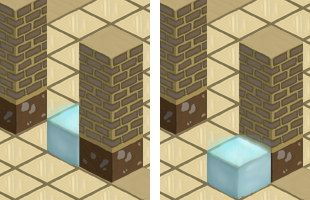
\includegraphics[scale=0.7]{Appendix4/figures/figure-1.png}
	\caption{This image shows a very early build of the game with \textsc{2d} isometric graphics. The blue block represents a player. On the left, the player is obscured by an object; on the right, the player is in front of it.\label{figure_1}}
\end{figure}

An online, multiplayer game based in the browser, utilising \textsc{html5} canvas and JavaScript for the client and Python for the server. It will be played similarly to the table-top roleplaying game \textit{Dungeons \& Dragons}, with a Game Master and several players.

The players will interact with the world in two modes or states. The first is a free-roaming state that operates in real-time. In this state, players will be allowed to interact with the world and the objects and characters within it with relative freedom. The rules that govern them will be loose and mostly describe the interactions of objects with other objects. For example, a magic spell that creates fire would have a heat attribute, and a door made of wood would have a burning point attribute. When they met, if the heat was greater than the burning point, the door would be set on fire.

The other state is the combat state. Players in this state will be locked into a turn-based system where they can only move and perform actions in a limited amount during their turn. Opponents can be creatures or other characters—both player and non-player—and will take their own turns to perform actions. Non-player characters and creatures will be operated by the Game Master. All characters and creatures will have attributes, such as health and mana (for magic), as well as a set of abilities that they can perform. If a character or creature reaches zero health it will have been killed and removed as an active element.

Each player will operate a single character and their view of the world and abilities within it will be defined by that character's location and abilities. If a character is too far away to see another character, then the player will also not see the other character. If a character cannot use magic spells, then the player will not be able to use them.

Player characters who are killed, either in battle or in some other way (perhaps they are killed by falling rocks in the free-roam state) are no longer playable. Players who lose their character may be removed from the game, become a spectator, be given an already existing character previously controlled by the Game Master or be allowed to make a new character.

The Game Master is not a player but rather the controller of the world. They will be able to interact with the world without limitations and be responsible for creating the world via a map editor, guiding the players around it, operating non-player characters and creatures in the world and set up events for the players. The Game Master will even be able to override the normal rules of the world. In the example of the fire spell and the door, the Game Master will be able to say that the door is not set on fire, even if it otherwise would have been.

The world will be presented to users using tile-based, \textsc{2d} isometric graphics (as seen in Figure \ref{figure_1}). It will consist of a planar terrain with objects, items and characters on top of it. Movement in the world will be done in 8 directions: up, down, left, right and diagonal. Characters and creatures will move from tile to tile, with only one able to be in a tile at any given time. However, each tile can hold many items (such as weapons, money, clothes). Objects will be varied, with those such as walls and pillars taking up a tile by themselves but objects such as chairs or chests of treasure that can be interacted with by characters may coexist in a tile with characters.

The players and Game Master will be able to communicate throught a textual chat system. In its most basic form, this will be a global chat that all users in the game can see. However, the ability to restrict chat to a local context or to an individual user would be nice.

Extra features that would enhance the project but are not mandatory include: voice chat system; multi-levelled maps with varying heights; random map generator; random creature/character generator; visual representation for character items (such as weapons, clothes, etc); and the ability for users to upload their own artwork for use in their games.

%==============================================================================
\section{Proposed tasks}
%==============================================================================
My proposed tasks to achieve a basic version of the project are as follows:

\begin{itemize}
	\item{Create basic client-side graphics engine, allowing a map to be rendered and a player to move around.}
	\item{Create basic multiplayer functionality, setting up the server and allowing multiple players to exist in the same map and move around within it.}
	\item{Add Game Master, who can select different characters to control.}
	\item{Add items and attributes to characters, allowing them to carry things and setting things up for the next task.}
	\item{Add combat state, allowing users to do more than walk around the world.}
	\item{Add attribute interactions in the free-roam state, allowing for the fire spell and wooden door interaction.}
	\item{Add map editor for the Game Master.}
\end{itemize}

%==============================================================================
\section{Project deliverables}
%==============================================================================
\begin{description}
	\item{\textbf{Game Client,} final `production' version.} This is what the users of the game will interact with, via a browser, allowing for both regular players and a Game Master, who is given the ability to create maps for the game.

	\item{\textbf{Game Server,} final `production' version.} This will be responsible for syncing the game between all the players and providing authoritative state to clients to help prevent cheating.

	\item{\textbf{Documentation.}} Basic guides for users that instruct them on how to operate the game from the Game Master and player perspectives.

	\item{\textbf{Final Report.}} Report detailing the system; the process of the system's creation from beginning to end; differences between the proposal and final system and explanations for those differences; full bibliography.
\end{description}

\fancypagestyle{plain}{%
   \fancyhead{} %[C]{Annotated Bibliography}
   \fancyfoot[C]{{\thepage} of \pageref{LastPage}} % except the center
   \renewcommand{\headrulewidth}{0pt}
   \renewcommand{\footrulewidth}{0pt}
}

\setemptyheader

\nocite{*} % include everything from the bibliography, irrespective of whether it has been referenced.

% the following line is included so that the bibliography is also shown in the table of contents. There is the possibility that this is added to the previous page for the bibliography. To address this, a newline is added so that it appears on the first page for the bibliography.
\addcontentsline{toc}{chapter}{Annotated Bibliography} % Adds References to contents page

%
% example of including an annotated bibliography. The current style is an author date one. If you want to change, comment out the line and uncomment the subsequent line. You should also modify the packages included at the top (see the notes earlier in the file) and then trash your aux files and re-run.
%\bibliographystyle{authordate2annot}
\bibliographystyle{IEEEannot}
\renewcommand{\bibname}{Annotated Bibliography}
\bibliography{References/references} % References file


\end{document}
